
%%%%%%%%%%%%%%%%%%%%%%%%%%%%%%
\section{Révolution quantique}
%%%%%%%%%%%%%%%%%%%%%%%%%%%%%%
%
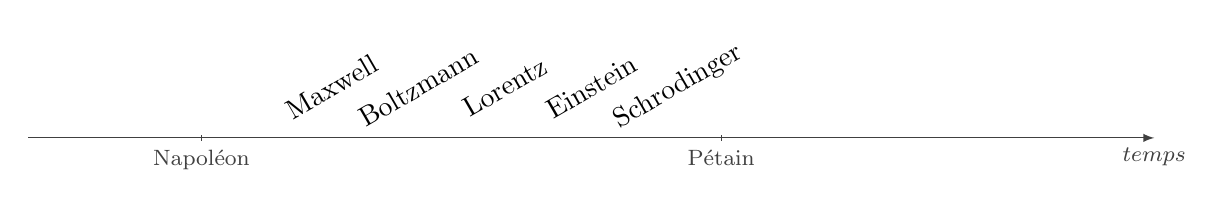
\begin{tikzpicture}
    \def\horizontal {5.5}
    \def\vertical {1.3}
\draw[-latex,color=darkgray] (17.7*\horizontal,0) -- (20.3*\horizontal,0);
\draw[shift={(20.3*\horizontal,0)},color=darkgray,thin]
                                   node[below] {\footnotesize $temps$};
%1769-1821
  \draw[shift={(18.10*\horizontal,0)},color=darkgray,thin] (0pt,1pt) -- (0pt,-1pt)
                                   node[below] {\footnotesize Napoléon};
%1856-1951
  \draw[shift={(19.3*\horizontal,0)},color=darkgray,thin] (0pt,1pt) -- (0pt,-1pt)
                                   node[below] {\footnotesize Pétain};
%1831-1879
\draw (18.4*\horizontal,0.5*\vertical) node [rotate=30]{Maxwell};
%1844-1906
\draw (18.6*\horizontal,0.5*\vertical) node [rotate=30]{Boltzmann};
%1853-1928
\draw (18.8*\horizontal,0.5*\vertical) node [rotate=30]{Lorentz};
%1879-1955
\draw (19*\horizontal,0.5*\vertical) node [rotate=30]{Einstein};
%1887-1961
\draw (19.2*\horizontal,0.5*\vertical) node [rotate=30]{Schrodinger};
\end{tikzpicture}
%
%
\subsection{Maxwell}

Les équations de Maxwell conduisent à l'unification des phénomènes magnétique, électrique et lumineux.

Les équations d'onde qui en découle unifient l'électromagnétisme avec la lumière, et font apparaître la constance de la vitesse de la lumière

\subsection{Boltzmann}

Ludwig Boltzmann développe la physique statistique en utilisant l'hypothèse atomique. Le succès de ses résultats conforte cette hypothèse. L'introduction de l'entropie statistique offre un éclairage des principes de la thermodynamique classique.

\subsection{Lorentz}
La transformations de Lorentz réconcilie la constance de la vitesse de la lumière avec le principe de relativité de Galilée.

\subsection{Einstein}
La présence de masse courbe l'espace temps, autrement dit les corps ne s'attirent pas.

\subsection{Schrödinger}
La fonction d'onde décrit le mouvement des quantons.
%%%%%%%%%%%%%%%%%%%%%%%%%%%%%%%%%%%%%%%%%%%%%%%%%%%%%%%%%%%%%%%%%%%%%%%%%%%%%%%%%%%%%
